\documentclass[12pt]{article}
\usepackage[margin=1in]{geometry}
\usepackage{natbib}
\usepackage{graphicx}
\usepackage{caption}
\usepackage{subcaption}
\usepackage{multirow}
\usepackage{longtable}
\usepackage{color}
\usepackage{hyperref}
\bibliographystyle{apalike}
\newcommand{\beginsupplement}{%
        \setcounter{table}{0}
        \renewcommand{\thetable}{S\arabic{table}}%
        \setcounter{figure}{0}
        \renewcommand{\thefigure}{S\arabic{figure}}%
     }
\newcommand{\citex}{\textcolor{red}{\bf CITE }}
\newcommand{\X}{\textcolor{red}{\bf X }}
\newcommand{\jri}[1]{\textcolor{red}{\emph{#1}}}
\newcommand{\dv}[1]{\textcolor{blue}{\emph{#1}}}

\begin{document}

\title{Evolutionary genomics of peach \\and almond domestication}

\author{\small\sfbf{Dianne Velasco$^{\S\dag}$, Mallikarjuna Aradhya$^{\dag}$, Jeffrey Ross-Ibarra$^{\S\ddag}$}\thanks{Corresponding author: Department of Plant Sciences, University of California, Davis, California 95616, USA. E-mail: \mbox{rossibarra@ucdavis.edu}} \\[0.3cm]
     \small\sf $^{\S}$Department of Plant Sciences, University of California, Davis, California 95616, USA,\\
     \small\sf $^{\dag}$USDA-ARS National Clonal Germplasm Repository, Davis, California 95616, USA,\\
     \small\sf $^{\ddag}$Center for Population Biology and Genome Center, University of California, Davis, \\ \small\sf California 95616, USA}

\date{\today}
\maketitle

\section*{Introduction}
%BACKGROUND ON SPECIES

\emph{Prunus} is a large genus in the family Rosaceae with approximately two hundred species, including multiple domesticated crops, such as almond, apricot, cherry, peach, and plum \citep{rehder1940manual, potter2011prunus}.
% approx 200 species shi2013phylogeny, citing rehder1940manual <- check out
% non-referenced 430 species in Wikipedia
%
Peach [\emph{P. persica} (Mill.) D. A. Webb] and almond [\emph{P. dulcis} (L.) Batsch] are sibling species found within the subgenus \emph{Amygdalus} sharing many morphological and physiological similarities, including perenniality, precocity, genome organization \citep{arus2012peach}, and genome size \citep{baird1994estimating}. 
% what did I mean by "early fruit development, "
%
The most striking differences between the species are mature fruit morphology and mating systems: peaches are harvested for their indehiscent fleshy mesocarp while almonds are harvested for the stony endocarp encased seeds obtained from within the leathery dehiscent mesocarp and exocarp. 
%
But almond and peach also differ for other traits, such as life span, chilling requirement, and adventitious root generation.
%
The natural life span of almonds may exceed 100 years \citep{gradziel2011origin},
% though no reference to a primary source in this review
% most literature sources describe commercial/production lifespan
% commercial: lifespan of 20-25 years, but this may be due to use of peach/peach-derived rootstocks and/or almond bearing decline and replacement as a management practice
flowering initiation requires only 400-600 hours chilling \citep{alonso2005determination}, 
% versus peach <650-1050 /citep{dozier1990hydrogen}
% perhaps it is actually lower considering the low chill peach cultivars
% look for additional sources
and poor adventitious root generation \citex when compared to the peach life span of 25-30 years \citex, 
%commercial production life span only or "wild" too?
600-1000 hours of required chilling \citex,
% can be far lower for low-chill varieties, approx. as low as 50, but more in the 100-450 hours range 
% Scorza & Okie (scorza1991peaches) state low chill are 150-500 hours, and most temperate are 650-950 hours
% high chill varieties are up to 1050-1100 hours
% 
%
and good adventitious rooting ability \citex. 
%chilling: qtl at distal end of LG1 had highest contribution to phenotypic variance in chilling (Bielenberg et al. 2004, referenced in Genetics, Genomics, and Breeding of Stone Fruits, chp 6)
%
Additionally, while \emph{Prunus} species generally exhibit gametophytic self-incompatibility, peach is fully self-compatible.

%DOMESTICATION
Domestication of almond and peach occurred approximately 5000 BP in the Fertile Crescent and China \citep{zohary2012domestication}, respectively, followed by global dissemination beginning before 2300 BP \citep{hedrick1917peaches, edwards1975almond, gradziel2011origin, zheng2014archaeological}. 
%
The few obvious traits associated with almond domestication are reduced toxicity, thinner endocarp, and increased seed size, while domestication in peach is characterized by diverse fruit morphology (size, color, texture, shape, etc.) and self-compatibility.
%
However, traits not typically associated with domestication but common to both, such as precocity, or solely with peach, such as relative ease of adventitious rooting, may have also been deliberately or incidentally selected during domestication. 
%
Unfortunately, efforts to identify wild progenitors of almond and peach by examining species relationships within the subgenus \emph{Amygdalus} have had mixed results \citep{mowrey1990isozyme, browicz1996genus, ladizinsky1999origin, aradhya2004molecular, bassi20081, zeinalabedini2010origin, verde2013high}. 
%
Given the uncertainty in identifying wild progenitors and the difficulties associated with long generation times, investigation of domestication using crossing experiments is impractical for almond and peach.
%
In contrast, inexpensive sequencing makes population genetic approaches (cf. \citealp{ross2007plant}) are an attractive option, enabling the identification of domestication loci and the genome-wide impacts of changes in mating system.   
%
Both domestication and mating system have been shown to shape genome diversity in annual species \citep{glemin2006impact, doebley2006molecular, slotte2013capsella}, but the impacts of these forces on tree species remains poorly understood \citep{mckey2010evolutionary, miller2011forest}.

%DOMESTICATION VERSUS SI/SC IN GENOME
In closely related species pairs with alternate mating systems, such as \emph{Arabidopsis thaliana} and \emph{A. lyrata} and \emph{Capsella rubella} and \emph{C. grandiflora} \citep{slotte2013capsella}, mating system is shown to significantly affect genome evolution, as evidenced by nucleotide diversity, linkage disequilibrium (LD), heterozygosity, genome size, repeat content, and genetic load.
%
We thus expect that that self-compatible peach has lower genome-wide diversity than self-incompatible almond.
%
However, domestication reduces genomic diversity genome-wide due to reduced effective population size \citex as well as localized regions important to domestication \citep{glemin2006impact, doebley2006molecular}. 
% \citep{charlesworth2001breeding}. 
%
\dv{Studies in perennials, particularly tree fruit crops, suggest they lose little genetic diversity due to domestication (reviewed in \citealp{miller2011forest}, p. 1399).}
%
Recent analysis of resequenced peach genomes indicates lower genetic diversity and higher LD across the genome compared to wild peach species \citep{verde2013high}, but the few resequenced almond genomes have not been similarly assessed. 
%
%STUDY PURPOSE AND SUMMARY
Here we present an evolutionary genomic analysis of the effects of domestication and mating system on genomic diversity in peach and almond, providing a model for future analysis of evolution and domestication in other tree species.
%
Understanding the impact of mating system on almond and peach evolutionary genomics expands the basic understanding of genome evolution in a perennial species pair with alternate mating systems. 
%is this a first for closely related perennial species pair with alternate mating systems? <-- DUNNO, THAT WOULD BE COOL!
%
Identification of candidate domestication loci will provide an opportunity to determine which loci in almond and peach were under selection, if any are in common, and to identify similarities or differences when compared to annual crops.
%
\section*{Materials and Methods}
%
\subsection*{Samples}
We analyzed a total of 14 almond and 32 peach genomes, including both public and newly resequenced data (Table \ref{samples}). 
%
For this study we resequenced nine \emph{P. dulcis}, one \emph{P. persica}, and one plum, \emph{P. cerasifera}, as outgroup species for analysis.
%
Fresh leaves and dormant cuttings collected from multiple sources (reference 1 in Table \ref{sampledetails}) and either desiccated with silica or refrigerated, respectively, followed by DNA isolation using a modified CTAB method \citep{doyle1987rapid}.
%
Paired-end 100bp sequences were generated for all samples on an Illumina HiSeq 2000. 
%
Of these samples, eight \emph{P. dulcis} were sequenced at the Vincent J. Coates Genomics Sequencing Laboratory at UC Berkeley from libraries prepared in our laboratory following an in-house protocol. 
DNA of the remaining four samples was submitted to BGI (Shenzen, China) for library preparation and sequencing at their facility.
% In the 'we sequenced' paragraph you need to provide PE 100, where they were sequenced, what average depth, and a citation for library prep (or if we paid someone to prep libraries)

% library prep section below seems awkward and out of place...
In-house sequencing library preparation requires quantifying the samples with Quanti-iT Picogreen dsDNA assay (Invitrogen, Life Technologies) and then fragmenting 1 $\mu$g of DNA with a Bioruptor (Diagenode) for \dv{11} cycles of 30 seconds ON and 30 seconds OFF per cycle. 
%
Resulting DNA fragment ends are then repaired with NEBNext End Repair (New England BioLabs) followed by the addition of deoxyadenosine triphosphate to the 3-prime ends with Klenow Fragment (New England BioLabs). 
%
Barcoded Illumina TrueSeq adapters (Affymetrix) were ligated to the A-tailed fragments with Quick Ligase (New England BioLabs). 
%
DNA was washed with sera-mags speed beads (Fisher Scientific) between each enzymatic step.  
%
Resulting libraries were quantified with Qubit (Life Technologies) and sized using a  BioAnalyzer DNA 12000 chip (Agilent Technologies) at UC Davis. 
%
The eight \emph{P. dulcis} sample libraries prepared in-house were sent to UC Berkeley (Berkeley, Qb3), multiplexed based on qPCR quantification, and paired-end sequenced to 100 bp in each direction on a single lane of a HiSeq2500 (Illumina).

Additionally, we utilized five resequenced \emph{P. dulcis} genomes from public sources, four from \citealt{koepke2013comparative} %(?)
the NCBI Sequence Read Archive (SRA) and one from the RosBREED group (\url{www.rosbreed.org}). 
%
We further downloaded thirty-one resequenced \emph{P. persica}, thirteen from the NCBI SRA (ten from \citealp{verde2013high} and three from \citealp{ahmad2011whole}) and eighteen from RosBREED.
%
%One wild peach species, \emph{P. ferganensis}, was publicly available from NCBI SRA \citep{verde2013high}. \jri{are we using this guy?} \dv{you suggested including it, but doesn't seem likely that it will be used}
%
\subsection*{Analysis}
\emph{Sequencing, Quality Control, and Mapping}

Sequences downloaded from RosBREED required additional pre-processing to match forward and reverse FASTQ file reads.
%supplementary methods for details?
%Pre-processing: concatenate the four lines per read ID for forward and reverse, use the ID prefix find the intersect, select the reads in each file with those prefixes, and finally decatenate (is that a word?) the reads into proper FASTQ files
%
The resulting FASTQ files were then processed in the manner described below.
%
All FASTQ files were trimmed of remnant adapter sequences using Scythe (\url{github.com/vsbuffalo/scythe}) and then further trimmed using base quality with Sickle (\url{github.com/najoshi/sickle}). 
%
Trimmed reads were then aligned to the peach v1.0 reference (\url{www.rosaceae.org}) using BWA-MEM \citep{li2013aligning} with a minimum seed length of 10 and internal seed length of 2.85.
% using -k 10 -r 2.85 parameters
% -k INT	minimum seed length [19]
% -r FLOAT	look for internal seeds inside a seed longer than {-k} * FLOAT [1.5]
% overall seed length remains the same as default; picked this up from P. Morrell
%
Using SAMtools and the SAMtools flagstat subprogram \citep{li2009sequence} we determined the depth for all genome sequence alignments.
\\
%\emph{SNP calling}
% Only if going to use them
% ANGSD to SweepFinder \citep{nielsen2005genomic} format would be interesting
%
%SNPs and \jri{did we call SNPs for anything??} \dv{SNPs were called, but not used at this time; included in case they are ever used}
%
\\
\emph{Diversity Evaluation}

Initial estimated genotype likelihoods called with ANGSD \citep{korneliussen2014angsd}. 
%
Inbreeding coefficients were estimated using \emph{ngsF} from the \emph{ngsTools} \citep{fumagalli2014ngstools} suite.
%
Genotype likelihoods were called utilizing the estimated inbreeding coefficients. 
%
Using ANGSD genotype likelihoods and posterior probabilities we calculated several population genetics statistics, such as Watterson's theta ($\theta_{W}$; \citealp{watterson1975number}) and pairwise nucleotide diversity ($\theta_{\pi}$; \citealp{nei1979mathematical}), and neutrality deviation tests, such as Tajima's D \citep{tajima1989statistical}, Fay and Wu's H \citep{fay2000hitchhiking}, and Zeng's E \citep{zeng2006statistical}.
\\
%
\\
\emph{Population Comparisons}

We treated peach and almond samples as belonging to two populations to understand population structure, assign population proportions, and determine population differentiation. 
% covar with ngsPopGen, admixture with NGSadmix, Fst with ANGSD
% perhaps put the software with the specific analysis instead of intro sentence
%
First we performed a principal component analysis (PCA) with \emph{ngsPopGen} \citep{fumagalli2014ngstools} to determine whether there was any underlying population structure.
%might show clear distinction between groups, possibly some overlap
%
Next we used \emph{NGSadmix} \citep{skotte2013estimating} to assign almond and peach population proportions (\emph{K} = 2) to individuals. 
%
We evaluated proportion assignment accuracy utilizing the sequence of a previously identified F1 peach-almond hybrid and a peach variety with almond ancestry in its pedigree four generations prior. 
% Gradziel, via Martinez-Garcia pers comm
Finally, we examined population differentiation using F$_{ST}$ as determined by ANGSD.
%1 kb windows, 200 bp steps
\\
\\
\emph{Identification of Selected Loci}

Genome-wide population genetics statistics (thetaPi, thetaW, Fay \& Wu's H, Zeng's E) were calculated in 1000 bp windows with 50 bp steps using the \emph{ngsTools} \citep{fumagalli2014ngstools} suite. 
%
Only windows with $>100$ bp were used for analysis; average values over particular annotations (e.g. genes) were calculated using bedtools \citep{quinlan2010bedtools}.
%
Putatively selected genes were identified by finding the 1\% and 5\% empirical quantiles of Zeng's E statistic \citep{zeng2006statistical}.
%
%
We analyzed these loci for gene ontology (GO) using the singular enrichment analysis tool and \emph{P. persica} protein IDs at the AgriGO website (\url{http://bioinfo.cau.edu.cn/agriGO/}).
%
%Determing shared loci and significance
% evaluation of gene annotations and any already suspected or known from function or location (Table S2?)
% overlap of pi, neutrality tests
%
%BEGIN TABLE
\begin{center}
\begin{longtable}{lccll}
\caption{\emph{P. dulcis}, \emph{P. persica} and outgroup species used in analyses.} \label{samples} \\
\hline \hline 
\multicolumn{1}{l}{\textbf{Species}} &
\multicolumn{1}{c}{\textbf{\emph{n}}} &
\multicolumn{1}{c}{\textbf{Avg. Depth}} &
\multicolumn{1}{l}{\textbf{Source}} &
\multicolumn{1}{l}{\textbf{Ref}}\\
\hline 
\endfirsthead

\multicolumn{5}{r}{{\bfseries \tablename\ \thetable{} -- continued from previous page}} \\
\hline
\multicolumn{1}{l}{\textbf{Species}} &
\multicolumn{1}{c}{\textbf{\emph{n}}} &
\multicolumn{1}{c}{\textbf{Avg. Depth}} &
\multicolumn{1}{l}{\textbf{Source}} &
\multicolumn{1}{l}{\textbf{Ref}} \\
\hline 
\endhead
%
\hline
\multicolumn{5}{r}{{Continued on next page}} \\
\hline \hline
\endfoot
%
\endlastfoot
%
	\emph{P. dulcis} &4 &7.76 &NCBI SRA &\citealp{koepke2013comparative}\\
	\emph{P. dulcis} &1 &2.20 &RosBREED &RosBREED$^{1}$\\
	\emph{P. dulcis} &8 &17.43 &UC Berkeley &this study$^{2}$\\
	\emph{P. dulcis} &1 &34.59 &BGI &this study$^{2}$\\
	\emph{P. persica} &10 &19.13 &NCBI SRA &\citealp{verde2013high} \\
	\emph{P. persica} &3 &13.78 &NCBI SRA &\citealp{ahmad2011whole} \\
	\emph{P. persica} &18 &1.53 &RosBREED &RosBREED$^{1}$ \\
	\emph{P. persica} &1 &37.36 &BGI &this study$^{2}$\\
	% ABC funded resequencing (performed at BGI)
%	\emph{P. fenzliana} &1 & &BGI &this study\\
	% UCD,ABC
%	\emph{P. ferganensis} &1 & &NCBI SRA &\citealt{verde2013high}\\
	\emph{P. cerasifera} &1 &35.02 &BGI &this study$^{2}$\\ \hline \hline
	% outgroup
	\multicolumn{5}{l}{$^{1}$ \url{ftp://ftp.bioinfo.wsu.edu/www.rosbreed.org/resequencing/Prunus_persica/}}\\
	\multicolumn{5}{l}{$^{2}$ newly resequenced sample(s)}
	% OR ftp://ftp.bioinfo.wsu.edu/species/Prunus_persica/RosBREED_Illumina/
\end{longtable}
\end{center}
% END TABLE
%
%add indicator whether sample was plant material or public sequence (reference does give some indication or possibly just put indication that when "this study" is the reference that it indicates that plant material was used)
%
\section*{Results}
%\subsection*{Quality Control and Mapping}

The aligned sequences had a mean mapped sequence depth of 10.71, which ranged from 1.14 to 37.36 (Table \ref{sampledetails}, Figure \ref{fig:depth}). %update depth figure, make supplementary
%
Genomes resequenced in this study had an average depth of 22.40, ranging from 14.47 to 37.36, while the depth of public sequences had an average depth of 7.92 ranging from 1.14 to 35.40.
%
Depth of all analyzed \emph{P. persica} sequences averaged 8.917 (1.138 to 35.358) while all \emph{P. dulcis} sequences averaged 14.808 (2.196 to 34.593).
% deposit scripts for data processing or extraction - deposit to github repo, add URL
%
\subsection*{Diversity and Population Comparisons}

Inbreeding values for almond and peach averaged 0.0275 0.3131 with ranges of 0.0030 to 0.2720 and 0.0040 to 0.8730, respectively.
%almond less inbred (average near zero, couple outliers - lower coverage), peach average approximately .25-.30.
%
Both diversity statistics indicated that almond was more diverse than peach, with genome-wide average $\theta_{\pi}$ of 0.0186 and 0.0035, respectively, and $\theta_{W}$ of \X and \X, respectively.
%
Mean per chromosome $\theta_{\pi}$ ranged from 0.0163 to 0.0219 in dulcis, and from 0.0028 to 0.0047 in persica.
% Are there interesting signals? Quantity? Where? Are there any interesting genes/loci?
%
Neutrality tests: Tajima's D, Fay and Wu's H, and Zeng's E \dv{yo, me! do this here!}
% Genome averages? Are there interesting signals? Quantity? Where? Are there any interesting genes/loci?
% Do any of the diversity statistics and neutrality tests overlap? Where? Are there any interesting genes/loci?
%
For the admixture results individuals were clearly assigned to either peach or almond populations (Figure \ref{fig:admix}). 
%
The previously identified peach-almond F1 hybrid was assigned as 0.4758 dulcis and 0.5242 persica, while the peach with introgressed almond ancestry was assigned as \X dulcis and \X persica.
%If samples are in the same order as the list of BAM files...
%PD15 Nonpareil is now 0.99999999282605944728 0.00000000717394056482
% whereas it was the same as other dulcis in previous test without PP12
%PP12 F8,1-42 0.00000000100000000000 0.99999999900000002828 (almond, peach; no different than rest of peaches) this seems odd for something with almond in pedigree only a few generations back
%TBD - RUNNING...
%

F$_{ST}$: unweighted 0.029449; weighted 0.668699; difference between them is whether it is the average of the ratio or ratio of $\Sigma$(numerator) and $\Sigma$(denominator).

% \jri{wait what? that big a difference just due to weighting?} \dv{yup, as we've discussed in meetings; your naive estimation based on pi was approximately 0.4, Malli's Fst for almond/peach based on AFLP was 0.446 \citep{aradhya2004molecular}}
%
\subsection*{Selected Loci and Gene Ontology}
Of the 27256 genes on chromosomes one through eight, dulcis and persica had 265 and 268 genes, respectively, in the 1\% quantile. 
%total genes on all chromosomes \& scaffolds: 27864\\
%
Twenty-nine of those genes, or approximately 11\%, are shared between dulcis and persica.
%
In the 5\% quantile dulcis and persica had 1325 and 1340 genes of interest, respectively, with 286 shared.
%
\dv{There is not nearly enough in this section... add information about interesting loci; describe the most interesting, or those that are known; a supplementary table; example figures of overlap of $\pi$, Tajima's D, Fay \& Wu's H, Zeng's E, and/or Fst for interesting areas, especially regions where signals are similar to regions like S-locus}
% 
%
\section*{Discussion}
%The what did we just learn, what does it all mean, and other stuff section
%Well, here are my crappy thoughts
Prior genome scans of peach by \cite{verde2013high} found low levels of genetic diversity compared to its wild relatives, \emph{P. kansuensis}, \emph{P. mira}, and \emph{P. davidiana}. 
%so what?
%
%\citep{cao2014comparative} - no wild relatives
%Genome-wide nucleotide diversity in persica and wild peaches (Verde et al. 2013)
% persica 0.0015 (ranged from 0.0011 to 0.0022)
% kansuensis 0.0008 (autogamous)
% davidiana 0.0048 (allogamous)
% mira 0.0013 (autogamous)
% N.B. only single samples of each species used
%
%\citealp{koepke2013comparative} looked at significant SNPs but not popgen stats with same public almond sequence data, cherry, and peach reference
%
Of these wild peach species, \emph{P. davidiana} is the only outcrossing one thus having a closer affinity with \emph{P. dulcis} \citep{aradhya2004molecular}. \dv{cite others regarding davidiana relationship to dulcis} 
%poor wording, more like peach with almond tendencies
%
\cite{verde2013high} found that \emph{P. davidiana} had the greatest nucleotide diversity of the species examined, approximately 3X the nucleotide diversity of \emph{P. persica}.
%
However, we found \emph{P. dulcis} to have double this level of nucleotide diversity confirming it is far more genetically diverse than any peach species.
% supposedly only SI wild peach
Considering their similar lengths of domestication, this finding suggests that mating system has had a greater impact on the reduction of peach genetic diversity than domestication.
% except the possible life span difference, except P. mira has been reported to live ~100 years \citep{bassi20081} or chapter 2 of same book, seem to recall there was no citation for the time period
%
While this difference in diversity between peach and almond has been known from analyses using multiple marker systems [e.g., isozyme \citep{mowrey1990isozyme, byrne1990isozyme}, microsatellite \citep{martinez2003extended}, and AFLP \citep{aradhya2004molecular} markers], this study marks the first simultaneous whole genome comparisons using multiple individuals from both species.
%
%
Therefore this study does support previous studies as having been good estimations of nucleotide diversity. 

% \jri{are there candidates for the S locus? can we at least zoom in on the arm to see if there are obvious sweeps (low diversity, negative E, high Fst between species)?}
\dv{broadly recap the findings, but more importantly their significance and what they bring to the understanding of domestication in tree crops, almonds, peaches}
\dv{there are expected differences, such as at the S-locus. What else is expected? Sweet/bitter kernel locus: less diverse in dulcis than persica; Caveats: it is dominant allele so may be in het state in some individuals sampled; there is no selection for sweet allele in peach, if one is present in species, possibly normal (background) or v low diversity (if fixed b/c adaptive or something) at locus. Flower color: generally pink in persica and white in almond (white likely ancestral b/c most common color across Prunus) so lower or higher diversity in peach compared with almond? Some variability is present in peach flower color (e.g., light pink to deep pink or nearly red). is it fixed in almond? What if anything was unexpected, whether in shared or unshared loci, and does it make sense?}
%
We found \X genes of interest in peach and \X in almond from the 1\% and 5\% quartile ranges, with \X shared.
%
Peach and almond also share more genes of interest in common than expected due to random chance.
% Simple Chi-square puts probability near zero
%
Interesting they differed in genes related to/important for \X processes in peach and \X processes in almond.
%
These unshared, but still important, genes are likely to account for the differentiation of these closely related domesticated species.
% poor writing

One of the primary questions regarding domestication of perennial crops, particularly tree crops, is its genetic basis \citep{miller2011forest}. %and distinguishing it from other factors such as life history, hybridization, vegetative propagation
%
Here we have examined two closely related domesticated tree species with alternate mating systems in an attempt to tease apart the genomic signatures of domestication and mating system in order to better understand these processes in perennial species.
%
\dv{so what did we find? how does it differ, if it does, from what we might expect in annual species?}
%
Potential uses of information: identify diversity in loci within germplasm collection(s), MAS (particularly juvenile selection), further investigate non-annotated loci of interest to determine function (if any)
%
%
\dv{Potential breeding application of information}
%
%Peach Dissemination Records
% Persia 332 BC, Rome 79 AD, France 530 to 784 AD, & Americas 16th c Spain/England
%
%Nice peach generation time description:
% "a peach falling to the ground brings a peach tree that shall bear in three years, or sometimes sooner"
% Hedrick p45 quoting John Lawson (1700)
% Lawson also described the peach tendency of overabundant fruit produced: "They generally bear so full that they break great part of their limbs down"
% Lawson's statements also suggest the degree of inbreeding in Indian/American peaches: "we generally raise this fruit from the stone, which never fails to bring the same fruit" Hedrick p46
% grafting in the Americas was becoming more common practice by the end of the 18th century (Hedrick p57)
%
%Almond: Turkestan and Uygurs
% Wikipedia regarding Turkestan: "includes [parts to all of] present-day Turkmenistan, Kazakhstan, Uzbekistan Kyrgyzstan, and Xinjiang ("Chinese Turkestan")" and "acquired its "Turkic" character from the 4th to 6th centuries AD with the incipient Turkic expansion" although the Turkic peoples are purported to originate in the Altai Mountains (north of the east end of the Taklamakan Desert and west of the Gobi Desert) currently in China (?; Kashgar?) and origin of Uygur peoples
% Uygurs have a strong affiliation with almond, but their traditions are similar to those of Western Asia and Mediterranean Europe, so West to East or East to West?
% The Taklamakan Desert, or rather oases throughout, funneled the various silk routes through that desert and surrounding mountain ranges
% DV: Likely almond spread east with the "Turkic expansion" possible that the almond reverence and traditions spread with them
%
%Domestication in plants is often associated with
% increased size and morphological diversity of the harvested organ
% reduced seed dispersal
% adaptation to disturbed environments
% reduced toxicity, selfing, photoperiod insensitivity, etc.
% \citep{doebley2006molecular}
% 
%Only a few of these traits are noted in almond or peach
% Almond: seed size in almond, sweet kernels
% Peach: fruit size & color, range of bloom/maturity dates
% what about other tree crops? (Review Miller & Gross paper)
%
%Peach
% ~230 Mb (<2X \emph{Arabidopsis thaliana}) \citep{verde2013high}
% 8 chromosomes
% self-compatible
% seed to seed in 3 years
% model system for \emph{Prunus}
% low genetic diversity
%
%Almond
% 300 Mb; cytology estimate
% similar to pre-sequence estimates of peach \citep{arumuganathan1991nuclear}
% 8 chromosomes
% seed to seed ~3 years
% self-incompatible
% genetic diversity higher than peach
% not aware of LD information/analyses
%
%subgenus \emph{Amygdalus}
% species are diploid
% genetic and QTL mapping of TxE $F_{2}$ pop suggests similar genomic structure \citep{dirlewanger2004comparative}
% peach $F_2$ genetic maps had poor resolution \citep{arus2012peach, joobeur1998construction, aranzana2003set, dirlewanger2004comparative, dominguez2003plant} prob due to high LD \citep{verde2013high}
% much needed expansion of understanding these processes in perennial crops \citep{miller2011forest}
% resource for breeding
%

\section*{Aknowledgements}
%May ask Dan Potter, Tom Gradziel, and David Neale for comments
Support for DV provided by the McDonald Endowment for UC Davis Plant Sciences Graduate Student Research Assistantships and the Almond Board of California (ABC; grant HORT16-Aradhya/Ledbetter). 
%
Resequencing funded by the ABC (grant HORT16-Aradhya/ Ledbetter) and a Henry A. Jastro Research Fellowship. 
%
Resequencing funded by the Henry A. Jastro Research Fellowship was used the Vincent J. Coates Genomics Sequencing Laboratory at UC Berkeley, supported by NIH S10 Instrumentation Grants S10RR029668 and S10RR027303.
%
\pagebreak
%\bibliographystyle{apalike} %can use here and not in header
\bibliography{references.bib}
%
%FIGURE EXAMPLE
%demographic effects (Figure \ref{fig:peach}) can impact deleterious allele distro
%
\pagebreak
\begin{figure}[b]
\centering
   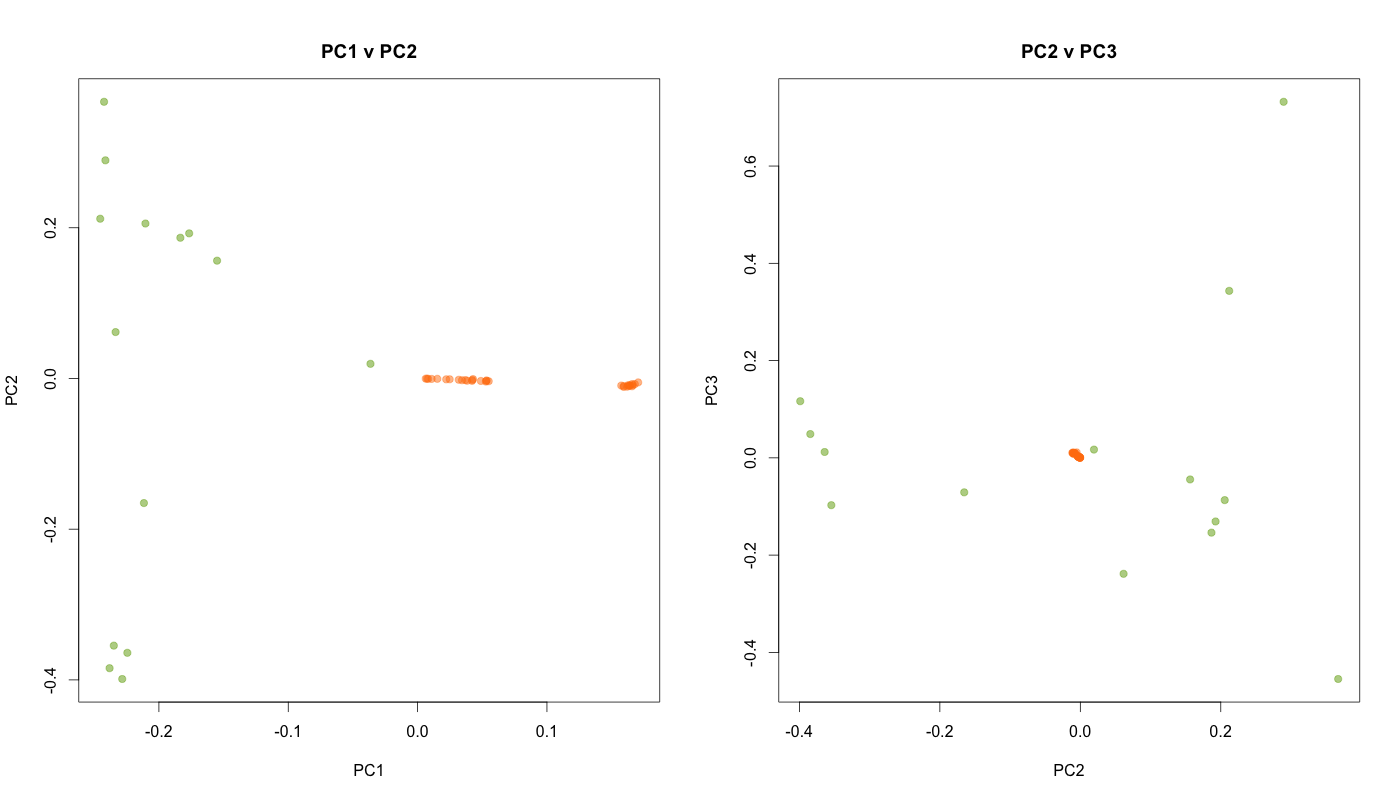
\includegraphics[width=0.8\textwidth]{pca.png}
  \caption{Principle component analysis plot of almond (green) and peach (orange) samples in the study. As evidenced by the PC2 vs PC3 plot (right), the second and third principle components only further differentiate almond samples but not peach samples. NOTE: low coverage samples cluster together near the center.}
  \label{fig:pca}
\end{figure}
%
\begin{figure}[b]
\centering
   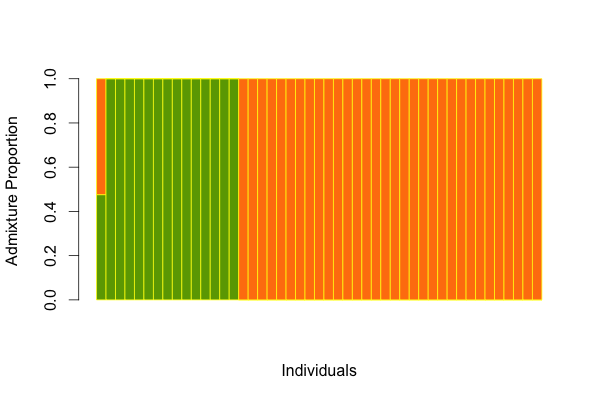
\includegraphics[width=0.8\textwidth]{Admixture_test.png}
  \caption{Proportion population assignment plot of almond (green) and peach (orange). The leftmost sample is an F1 hybrid between almond and peach.}
  \label{fig:admix}
\end{figure}
%
\pagebreak
%
%
\beginsupplement
\section*{Supplementary Data}
%
\begin{figure}[b]
\centering
   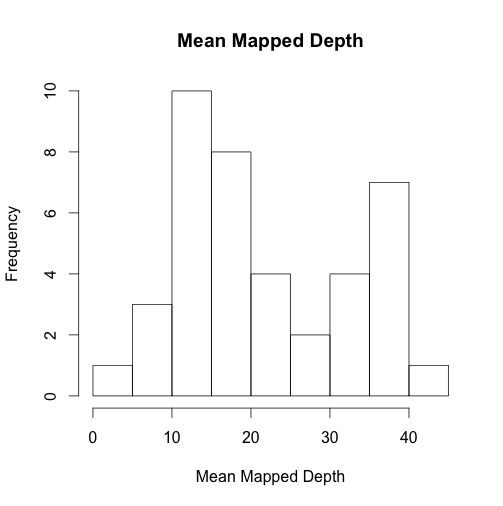
\includegraphics[width=0.8\textwidth]{depthBQ20MQ30.png}
  \caption{Mean mapped depth of all sequences, including those not used in this analysis \dv{UPDATE OR REMOVE THIS FIGURE}}
  \label{fig:depth}
\end{figure}
%
\begin{center}
\begin{longtable}{llrllc}
\caption{P. dulcis, P. persica and related species used in analysis.} \label{sampledetails} \\
\hline \hline
\multicolumn{1}{l}{\multirow{2}{1.5cm}{\textbf{Sample ID}}} &
\multicolumn{1}{l}{\multirow{2}{3.5cm}{\textbf{Accession and/or Cultivar}}} &
\multicolumn{1}{c}{\textbf{Depth}} &
\multicolumn{1}{l}{\textbf{Origin}} &
\multicolumn{1}{l}{\textbf{Source}} &
\multicolumn{1}{c}{\textbf{Ref}}\\ \\
\hline 
\endfirsthead

\multicolumn{6}{r}{{\bfseries \tablename\ \thetable{} -- continued from previous page}} \\
\hline 
\multicolumn{1}{l}{\multirow{2}{1.5cm}{\textbf{Sample ID}}} &
\multicolumn{1}{l}{\multirow{2}{3.5cm}{\textbf{Accession and/or Cultivar}}} &
\multicolumn{1}{c}{\textbf{Depth}} &
\multicolumn{1}{l}{\textbf{Origin}} &
\multicolumn{1}{l}{\textbf{Source}} &
\multicolumn{1}{c}{\textbf{Ref}} \\ \\ \hline 
\endhead
%
\hline \multicolumn{6}{r}{{Continued on next page}} \\ \hline \hline
\endfoot
%
\endlastfoot
%
	\multicolumn{6}{l}{\emph{P. dulcis}}  \\
	%PD01 &DPRU 2578.2 &30.46 &NCGR &this study\\
	% Almond Board resequencing (BGI)
	% Not included because it appears to be possible F1 of peach x almond (or reverse)
	PD02 &‘Tardy Nonpareil’ &34.59 &USA &UCD &1\\
	%Almond Board resequencing (BGI)
	PD03 &DPRU 1791.3, BE-1609 &17.93 &Turkey &USDA NCGR &1\\
	%Jastro resequencing (performed at UC Berkeley)
	PD04 &DPRU 2374.12 &16.77 &Iran &NCGR &1\\
	%Jastro resequencing (performed at UC Berkeley)
	PD05 &DPRU 1456.4, Badam &15.90 &Pakistan &USDA NCGR &1\\
	%Jastro resequencing (performed at UC Berkeley)
	PD06 &DPRU 2301, Tuono &17.23 &Italy &USDA NCGR &1\\
	%Jastro resequencing (performed at UC Berkeley)
	PD07 &DPRU 1462.2 &19.38 &Pakistan &USDA NCGR &1\\
	%Jastro resequencing (performed at UC Berkeley)
	PD08 &DPRU 1207.2 &14.47 &Uzbekistan &USDA NCGR &1\\
	%Jastro resequencing (performed at UC Berkeley)
	PD09 &DPRU 2331.9 &17.17 &China &USDA NCGR &1\\
	%Jastro resequencing (performed at UC Berkeley)
	PD10 &DPRU 0210, Languedoc &20.63 &France &USDA NCGR &1\\
	%Jastro resequencing (performed at UC Berkeley)
	PD11 &S3067 &6.64 &Spain &SRR765861 &2\\
	% resequenced at WSU by Amit Dhingra
	PD12 &D05-187 &4.72 &Spain &SRR765850 &2\\
	% resequenced at WSU by Amit Dhingra
	PD13 &Lauranne &13.00 &Spain &SRR765838 &2\\
	% resequenced at WSU by Amit Dhingra
	PD14 &Ramillete &6.69 &Spain &SRR765679 &2\\
	% resequenced at WSU by Amit Dhingra
	PD15 &Nonpareil &2.20 & USA&RosBREED &5\\
	\\
	\multicolumn{6}{l}{\emph{P. persica}}  \\ % format italics
	%PP01 &Lovell &81.14 &USA &SRR502985 &3\\
	% resequenced doubled haploid
	PP02 &Yumyeong &22.37 &Korea &SRR502994 &3\\
	PP03 &Shenzhou Mitao &11.19 &N China &
	\multirow{2}{1cm}{SRR502993, SRR502992} &3\\
	%honey peach
	\\
	PP04 &Sahua Hong Pantao &14.46 &S China &
	\multirow{2}{1cm}{SRR502991, SRR502990} &3\\
	%flat peach
	\\
	PP05 &Quetta &12.64 &Pakistan &
	\multirow{2}{1cm}{SRR502989, SRR502987} &3\\
	\\
	PP06 &Oro A &25.78 &Brazil &SRR502986 &3\\
	%
	PP07 &IF7310828 &12.75 &Italy &
	\multirow{2}{2cm}{SRR503001, SRR503000} &3\\
	\\
	PP08 &GF305 &18.68 &France &SRR502983 &3\\
	%
	PP09 &F$_{1}$ Contender $\times$ Ambra &15.57 &Italy &SRR502997 &3\\
	% peach x nectarine both P. persica
	%
	PP10 &Earligold &35.40 &USA &
	\multirow{2}{1cm}{SRR502996, SRR502995} &3\\
	%
	\\
	%
	PP11 &Bolero &22.42 &Italy &SRR501836 &3\\
	%
	% PP12 &F8,1-42 &11.88 &USA &SRR068361 &4\\
	% Nonpareil almond in pedigree
	% use for introgression investigation
	PP13 &Georgia Belle &13.13 &USA &SRR068359 &4\\
	%
	PP14 &Dr. Davis &14.44 &USA &SRR068360 &4\\
	%
	PP15 &Lovell &37.36 &USA &UCD &1\\
	% originally a canning variety selected ~1882
	% currently used as rootstock and/or control for disease screening
	% FPS, ABC
	% duplicate cultivar, BGI sequenced at higher depth
	PP16 &DPRU 1190, Admiral Dewey &1.61 &USA &RosBREED &5\\
	% aka PI 673525; introduced 1899
	PP17 &Babcock &1.74 &USA &RosBREED &5\\
	% introduced 1897
	PP18 &Bolinha &1.91 &Brazil &RosBREED &5\\
	% released 1985
	% parentage: prob OP Aldrighi
	% (Raseira et al. 1992;
	% http://hortsci.ashspublications.org/content/27/11/1154.full.pdf)
	% considered resistant to brown rot (Monilinia fructicola); low chill
	PP19 &DPRU 2142, Carman &1.34 &USA &RosBREED &5\\
	% Planted 1889 from OP seed (unknown variety) by J. W. Stubenrauch, Mexia, TX
	% data entry error listed as Carmen in GRIN; PI book has Carman
	% http://sun.ars-grin.gov:8080/npgs_public/prodweb.pdf0?in_vol=33&in_suffix=&in_page=052
	% PI 673586; cultivar original PI 34673 assigned 1912
	PP20 &Chinese Cling &1.28 &China &RosBREED &5\\
	%introduced 1850; founder several cultivars
	PP21 &Diamante &1.85 &Brazil &RosBREED &5\\
	%predominant canning cultivar in Brazil per Okie (year & pub TBD)
	PP22 &Dixon &1.28 &USA &RosBREED &5\\
	% Introduced in 1956
	% http://www.google.com/patents/USPP13911
	% early cling peach
	%PP23 &Dr. Davis &1.23 &USA &RosBREED &5\\
	% duplicate cultivar
	PP24 &DPRU 0589, Early Crawford &1.98 &USA &RosBREED &5\\
	%introduced before 1832
	PP25 &Elberta &1.26 &USA &RosBREED &5\\
	%introduced ~1889; OP sdlg of 'Chinese Cling’
	PP26 &Florida Prince P138 &1.48 &USA &RosBREED &5\\
	%low chill cultivar; introduced in 2009
	%PP27 &Georgia Bell &3.89 &USA &RosBREED &5\\
	%(aka ‘Georgia Belle’ and ‘Belle of Georgia’
	% introduced ~1875; OP sdlg of Chinese Cling)
	% duplicate cultivar
	PP28 &JH Hale &1.73 &USA &RosBREED &5\\
	%male sterile; introduced 1912
	%PP29 &Lovell &2.68 &USA &RosBREED &5\\
	PP30 &Mayflower &1.14 &USA &RosBREED &5\\
	%introduced 1909
	PP31 &Nemaguard &1.58 &USA &RosBREED &5\\
	%rootstock; rumored to have P. davidiana in pedigree
	PP32 &O'Henry &1.82 &USA &RosBREED &5\\
	%plant patent 2.964 1/27/1970; OP sdlg Merrill Bonanza; discovered 1960
	PP33 &Okinawa &1.55 &Japan &RosBREED &5\\
	% Sharpe 1957
	% http://fshs.org/proceedings-o/1957-vol-70/320-322%20%28SHARPE%29.pdf
	% from 1953 seed lot, different seedlings
	% unsure if only one of these is what is now called 'Okinawa'
	% has nematode resistance
	% used in hybrid combination with Harrow's Blood (F2s) as rootstock
	PP34 &Oldmixon Free &1.99 &USA &RosBREED &5\\
	% introduced 1832
	% Sir John Oldmixon in the mid 18th century wrote of peach in the Carolinas (Hedrick p50)
	PP35 &Rio Oso Gem &1.21 &USA &RosBREED &5\\
	% introduced 1933
	% developed in Rio Oso, California, Sierra Nevada foothills
	% https://www.slowfoodusa.org/ark-item/rio-oso-gem-peach
	PP36 &DPRU 2179, Slappey &1.24 &USA &RosBREED &5\\
	% aka ‘Slappy’ in GRIN; introduced 1903
	PP37 &DPRU 0941, St. John Yellow &1.14 &USA &RosBREED &5\\
	% introduced 1860s
	% some variety history at
	% http://gapeaches.org/about-us/father-of-the-ga-peach-industry/
	\\
	\multicolumn{6}{l}{Other \emph{P. cerasifera}}  \\
%	\multicolumn{6}{l}{Other \emph{Prunus} species}  \\
	% Almond Board resequencing (performed at BGI)
%	PF01 &\emph{P. fenzliana} &33.80 &\emph{unk.} &UCD &1\\
	% UCD,ABC
%	PG01 &\emph{P. ferganensis} &12.76 &Fergana Valley &
%	\multirow{2}{1cm}{SRR502999, SRR502998} &3\\
%	\\
	PC01 & DPRU 0579, Myrobalan &35.02 &USA &USDA NCGR &1\\
	%outgroup
 \hline \hline
	%
	%NCBI SRA
	%note that the SRR IDs are from NCBI SRA
	%GDR/RosBREED (ftp://ftp.bioinfo.wsu.edu/species/Prunus_persica/RosBREED_Illumina/)
	\multicolumn{6}{l}{\textbf{References:} $^{1}$ this study; $^{2}$ \citealp{koepke2013comparative}; $^{3}$ \citealp{verde2013high}; $^{4}$ \citealp{ahmad2011whole};}\\
	\multicolumn{6}{l}{$^{5}$ \url{ftp://ftp.bioinfo.wsu.edu/www.rosbreed.org/resequencing/Prunus_persica/}}\\
	\multicolumn{6}{l}{\textbf{Abbreviations:} UCD - University of California, Davis; USDA NCGR - United States}\\
	\multicolumn{6}{l}{Department of Agriculture National Clonal Germplasm Repository}
\end{longtable}
\end{center}
%
\pagebreak
% SHARED GENES
%
\begin{center}
\begin{longtable}{llll}
\caption{List of genes with low Zeng's E score shared between \emph{P. dulcis} and \emph{P. persica}} \label{sampledetails} \\
\hline \hline
\multicolumn{1}{l}{\textbf{Gene ID}} &
\multicolumn{1}{l}{\textbf{Annotation}} &
\multicolumn{1}{l}{\textbf{1\%}} &
\multicolumn{1}{l}{\textbf{5\%}}\\
\hline 
\endfirsthead

\multicolumn{4}{r}{{\bfseries \tablename\ \thetable{} -- continued from previous page}} \\
\hline 
\multicolumn{1}{l}{\textbf{Gene ID}} &
\multicolumn{1}{l}{\textbf{Annotation}} &
\multicolumn{1}{l}{\textbf{1\%}} &
\multicolumn{1}{l}{\textbf{5\%}} \\ \hline 
\endhead
%
\hline \multicolumn{4}{r}{{Continued on next page}} \\ \hline \hline
\endfoot
\hline \hline
\endlastfoot
%INCOMPLETE
%BRILLIANT IDEA - PREPARE IN EXCEL, WITH CELL DIVITERS, SAVE AS TEXT, COPY/PASTE
% ANNOTATIONS ALSO IN EXCEL FORMAT
% keep Zeng score? Sort by score? Note if 1% & 5% differently (for example, X and -)
	ppa000008m & & &Y \\
	ppa000009m & & &Y \\
	ppa000017m & & &Y \\
	ppa000033m & & &Y \\
	ppa000042m & & &Y \\
	ppa000051m & & &Y \\
	ppa000060m & & &Y \\
	ppa000069m & & &Y \\
	ppa000087m & & &Y \\
	ppa000098m & & &Y \\
	ppa000128m & & &Y \\
	ppa000151m & & &Y \\
	ppa000152m & & &Y \\
	ppa000208m & & &Y \\
	ppa000218m & & &Y \\
	ppa000246m & & &Y \\
	ppa000270m & & &Y \\
	ppa000282m & & &Y \\
	ppa000293m & & &Y \\
	ppa000320m & & &Y \\
	ppa000328m & & &Y \\
	ppa000332m & & &Y \\
	ppa000333m & & &Y \\
	ppa000344m & & &Y \\
	ppa000366m & & &Y \\
	ppa000395m & & &Y \\
	ppa000438m & & &Y \\
	ppa000473m & & &Y \\
	ppa000474m & & &Y \\
	ppa000499m & & &Y \\
	ppa000506m & & &Y \\
	ppa000507m & & &Y \\
	ppa000518m & & &Y \\
	ppa000595m & & &Y \\
	ppa000613m & & &Y \\
	ppa000615m & & &Y \\
	ppa000618m & & &Y \\
	ppa000624m & & &Y \\
	ppa000654m & & &Y \\
	ppa000734m & & &Y \\
	ppa000759m & & &Y \\
	ppa000819m & & &Y \\
	ppa000823m & & &Y \\
	ppa000871m & &Y &Y \\
	ppa000874m & & &Y \\
	ppa000889m & &Y &Y \\
	ppa000975m & & &Y \\
	ppa001014m & &Y &Y \\
	ppa001036m & &Y &Y \\
	ppa001053m & & &Y \\
	ppa001110m & &Y &Y \\
	ppa001188m & & &Y \\
\end{longtable}
\end{center}
%\endsupplement
\end{document}